% THIS IS SIGPROC-SP.TEX - VERSION 3.0
% WORKS WITH V3.1SP OF ACM_PROC_ARTICLE-SP.CLS
% JUNE 2007
%
% It is an example file showing how to use the 'acm_proc_article-sp.cls' V3.1SP
% LaTeX2e document class file for Conference Proceedings submissions.
% ----------------------------------------------------------------------------------------------------------------
% This .tex file (and associated .cls V3.1SP) *DOES NOT* produce:
%       1) The Permission Statement
%       2) The Conference (location) Info information
%       3) The Copyright Line with ACM data
%       4) Page numbering
% ---------------------------------------------------------------------------------------------------------------
% It is an example which *does* use the .bib file (from which the .bbl file
% is produced).
% REMEMBER HOWEVER: After having produced the .bbl file,
% and prior to final submission,
% you need to 'insert'  your .bbl file into your source .tex file so as to provide
% ONE 'self-contained' source file.
%
% Questions regarding SIGS should be sent to
% Adrienne Griscti ---> griscti@acm.org
%
% Questions/suggestions regarding the guidelines, .tex and .cls files, etc. to
% Gerald Murray ---> murray@acm.org
%
% For tracking purposes - this is V3.0SP - JUNE 2007

\documentclass{sig-alternate-10pt}

%\usepackage{graphicx}
\usepackage{paralist}
\newenvironment{mylisting}
{\begin{list}{}{\setlength{\leftmargin}{1em}}\item\scriptsize\bfseries}
{\end{list}}

\begin{document}

\title{{\ttlit Ratpack}: In-Place Aggregation of Sensor Data \titlenote{Submitted in partial fulfilment of requirements for the Sensor Networks Lab praktikum, SS07, RWTH Aachen}
}

\numberofauthors{2}
\author{ 
\alignauthor
Siddhu Warrier \\
\affaddr{European Masters in Informatics in Net-Centric Informatics}\\
\affaddr{Lehrstuhl f\"ur Informatik, RWTH Aachen}\\
\affaddr{Aachen, Germany}\\
\email{s.warrier@sms.ed.ac.uk}
\alignauthor
Galiia Khasanova \\
\affaddr{European Masters in Informatics in Embedded Systems Informatics}\\
\affaddr{Lehrstuhl f\"ur Informatik, RWTH Aachen}\\
\affaddr{Aachen, Germany}\\
\email{galiia.khasanova@rwth-aachen.de}
}

\maketitle
\begin{abstract}
Bayesian inference is a candidate to perform classification of collected sensor data in networks of intermittently-connected nodes, in order to minimise requirements. A demonstrator was developed on the Tmote Sky motes to prove the suitability of Bayesian inference. Future work includes deployment on sensor nodes with multiple sensors, the reduction of the size of the conditional probability matrix, and routing in intermittently connected networks.
\end{abstract}

% A category with the (minimum) three required fields
\category{E.2}{Data Storage Representations}{Data Classification}
%A category including the fourth, optional field follows...
\category{C.2.4}{Computer-Communication Networks}{Distributed Systems}

\terms{Bayesian Inference in Wireless Sensor Networks}

\keywords{wireless sensor networks, data classification, bayesian inference} % NOT required for Proceedings

\section{Introduction}

The aim of the RatPack
project\footnote{http://ds.informatik.rwth-aachen.de/research/projects/\\ratpack} -
a part of which was implemented during the course of this work - is to analyse
animal ecological and social networks using programmable sensor nodes. To this
end, it is envisioned to place sensor nodes on rats, and to collect sensor data
off them in order to understand rat behaviour. 

Sensor nodes have constraints on size \cite{SensorSurveyAkyildiz:2002}; thereby limiting memory capacity. Therefore, the amount of collected sensor data that
can be stored on the sensor node is limited. Additionally, connectivity among
nodes deployed on the monitored animals may be sporadic, as a result of which a
large number of sensor readings may have to be collected over a long period of time. This necessitates the investigation of mechanisms to reduce the size of the collected data. The mechanism considered in this work was to perform aggregation of the collected data on the sensor nodes itself.

\subsection{In-Place Aggregation of Sensor Data} \label{subsec:InplaceAggregation}

Aggregation may be performed using two approaches:

\begin{compactitem}
  \item Construction of a routing tree that periodically forwards sensor data to a sink.
  However, this may require transmissions across multiple hops, thereby producing a
  detrimental impact on power consumption. Additionally, this may not always be possible given the network is unlikely to be strongly connected at all times.
  \item Aggregation of collected sensor data (potentially from multiple sensors) on
  the sensor node.
\end{compactitem}

The rest of this paper discusses work on performing processing collected sensor
data and converting them into discrete Sensor Node States (SNSes), which can
be stored more
efficiently in memory. The conversion of data into states  is performed on
the basis of information on animal behaviour collected from biologists.

Two mechanisms may be potentially used to infer events from collected sensor
data:

\begin{compactitem}
  \item \emph{Using a Rule-based System:} The biologists observing rat behaviour
  define rules that would specify the SNS, given the previous SNS and the collected
  sensor data. 
  \item  \emph{Using Bayesian Learning and Bayesian Inference:} Bayesian
  Learning is used to learn the probability of the occurrence of a given SNS, given
  a large set of training data that maps sensor readings to SNSes. Following this,
  Bayesian Inference is used to determine the
  SNS likely to occur and its associated probability, given sensor readings.  
\end{compactitem} 

\subsection{Clustering Sensor Data into States} \label{subsubsec:Clustering}

Irrespective of the inference approach chosen, it is necessary to discretise
sensor data read into a set of states. This is done as follows:

\emph{Assumption}: Sensor data is scalar. \\ \\
\noindent
Let the sensors on each mote be $S_1, S_2, S_3$\ldots$S_{n_{sensor}}$, where
$n_{sensor}$ is the number of sensors.\\ \\
\noindent
Let sensor $S_i$ take scalar values in the range
$[x_0$,$x_1$,$x_2$\ldots$x_k]]$ for any arbitrary value of
$k$ such that $k \leq N$, where $N$ is
defined as the number of possible readings that may be obtained from the sensor \footnote{$N = \infty$, if a sensor produces real values (ignoring limits on reading
precision)}.\\ \\
\noindent
Let a single scalar \textbf{state} value, $St_{lm}$, be assigned to all sensor
readings with values in the interval $[x_l, x_m]$. \\ \\
\noindent
This results in a reduction in the space of sensor readings, $N$,
to $k-1$ discrete values.

\subsection{Rule-based Systems}

This section describes the first of the two aggregation mechanisms described in
Section \ref{subsec:InplaceAggregation}, namely, the rule-based system.

A rule-based system is a mechanism for knowledge representation wherein knowledge is
represented in terms of a set of rules that map from input (sensor
data) to output (SNS) \cite{RuleBasedAllison:2007,AIRichKnight:1990}. It
consists of several \emph{if-then} rules, facts, and an interpreter that controls the
application of the rules given the facts. Rule-based systems may be either
forward-chaining or backward-chaining. Forward chaining systems use the
provided facts recursively in order to derive conclusions, whereas Backward
Chaining systems work towards proving or disproving conclusions.

\subsubsection{Rule-based Systems for data aggregation}

The architecture of a rule-based system for data aggregation would require
domain experts to define rules of the form shown below, possibly using a visual
interface:\\ \\ \noindent
if ( ($Si.St$ OP $val_i$) \ldots LOP \ldots ($Sj.St$ OP $val_j$) ) \\
\{ \\
\hspace*{4 mm} \emph{Set SNS} \\
\}   
 
Rules may also take the current and previous SNSes into consideration when
determining the new SNS. The disadvantages of this approach include:  
\begin{compactitem}
 \item A large number of rules have to be defined. 
 \item The rules have to be stored on the
sensor node, potentially requiring large amounts of space.
\end{compactitem}

\subsection{Bayesian Inference}

Bayesian inference is a mechanism for statistical inference wherein evidence or
observations (for e.g.: sensor readings) are used to update or infer the
probability of the truth of a hypothesis. It uses Bayes' theorem to derive a
numerical estimate of the degree of belief in a hypothesis, on the basis of the
evidence observed and the degree of belief in the hypothesis before the
observation of the evidence:

\begin{equation} \label{eqn:Bayes}
	P(H_{0}|e) = \frac{P(e|H_{0})P(H_{0})}{P(e)}
\end{equation} 

\noindent
where:\\
\noindent
$H_{0}$ is the hypothesis the degree of belief in which is being assessed,\\
\noindent
$P(H_{0})$ is the probability that the hypothesis is true, when not given the
evidence, and is referred to as the prior probability,\\
\noindent 
 $e$ is the observed evidence,\\
 \noindent
 $P(e)$ is the marginal probability of $e$, which may be defined as the probability of witnessing the new evidence $e$ given all mutually exclusive hypotheses and the corresponding conditional probabilities, \\
\noindent
$P(e|H_{0})$ is the conditional probability of the evidence observed occurring,
given the truth of the hypothesis, and\\
\noindent
$P(H_{0}|e)$ is the conditional probability of the hypothesis being true, given
the observed evidence, and is referred to as the posterior probability.

%The factor $\frac{P(E|H_0)}{P(E)}$ represents the impact the evidence has on the hypothesis $H_0$. 

\subsubsection{Generalisation}

Bayesian inference can be applied iteratively when the degree of belief in a hypothesis is affected by multiple pieces of evidence that are independent of each other.\\

Let the set of independent evidences be E, such that:

\begin{equation*}
E = [e_i|i = 1\ldots N_{ev}]
\end{equation*}

\noindent
where:\\
\noindent
$e_i$ is the $i^{th}$ piece of independent evidence, and\\
\noindent
$N_{ev}$ is the number of independent evidences.

Then, given the pieces of evidence are independent of each other,

\begin{equation} \label{eqn:P(E)}
P(E) = P(e_1,e_2\ldots e_{N_{ev}}) = P(e_1) \times P(e_2)\ldots \times P(e_{N_{ev}})
\end{equation}

\noindent
where $P(e_i)$ is the marginal probability of the occurence of the evidence $e_i$.\\ \\
\noindent
and,

\begin{equation} \label{eqn:P(E|H0)}
P(E|H_0) = P(e_1|H_0) \times P(e_2|H_0) \ldots \times P(e_{N_{ev}}|H_0)
\end{equation}

Using equations \ref{eqn:P(E)} and \ref{eqn:P(E|H0)}, equation \ref{eqn:Bayes} becomes:

\begin{equation} \label{eqn:BayesMote}
P(H_0|E) = \frac{\prod_{i=1}^{N_{ev}}P(e_i|H_0) P(H_0)}{\prod_{i=1}^{N_{ev}}P(e_i)}
\end{equation}

Thus, Bayesian inference can be used to derive the degree of belief in a hypothesis on the basis of multiple, independent pieces of evidence, thereby indicating its suitability for inferring the SNS given a number of independent sensor readings.

\subsubsection{Bayesian Network}

Bayesian networks \cite{ProbReasoningPearl:1998} are also referred to as Belief
networks, knowledge maps, and
probabilistic causal methods. They are used to model incompletely understood 
situations which necessitate probabilistic descriptions
\cite{BayesianCharniak:1991}. A Bayesian network uses Bayesian inference to describe the
relationship between the causes (evidence) and the effects (hypothesis).

In order to construct a Bayesian network for the application domain under
consideration, it is necessary to determine the probability of the occurrence of a
state, given the
sensor readings. This can be achieved by having domain experts provide a set of
training data of the form :

\begin{equation}
S_{1}.St, S_{2}.St, S_{3}.St,...S_{n_{sensor}}.St, SNS 
\end{equation}
\noindent
where:\\
\noindent
$S_{i}$ is the $i^{th}$ sensor,\\
\noindent
$S_{i}.St$ is the state of the $i^{th}$ sensor, and\\
\noindent
the sensor readings are independent of each other. 

The training data is provided as input to a Bayesian learning package which
constructs the Bayesian network. 

Let $\lambda$ be defined as a particular set of sensor readings such that:

\begin{equation} \label{eqn:Lambda}
\lambda = [S_1.St = x_1, S_2.St = x_2, \ldots , S_{n_{sensor}}.St = x_{n_{sensor}}]
\end{equation}
\noindent
where $\forall x_i $ are random states.

The probability of the sensor node being in an SNS, $SNS_{\alpha}$, given the set of sensor readings $\lambda$ (see equation \ref{eqn:Lambda}), can then be derived using equation \ref{eqn:BayesMote}, as follows:

\begin{equation}
P(SNS_{\alpha}|\lambda) = \frac{\prod_{i=1}^{n_{sensor}}P(S_i.St = x_i | SNS_{\alpha}) P(SNS_{\alpha})}{\prod_{i=1}^{n_{sensor}}P(S_i.St = x_i)}
\end{equation}

The prior probability, $P(SNS_{\alpha})$, the conditional probability, $P(S_i.St = x_i | SNS_{\alpha})$, and the marginal probability $P(S_i.St = x_i)$ are determined from the training data, by the Bayesian learning mechanism.

The Bayesian network thus constructed may be represented schematically as shown in Figure \ref{Fig1:BayesianNet}.

 \begin{figure}[h]
\centering
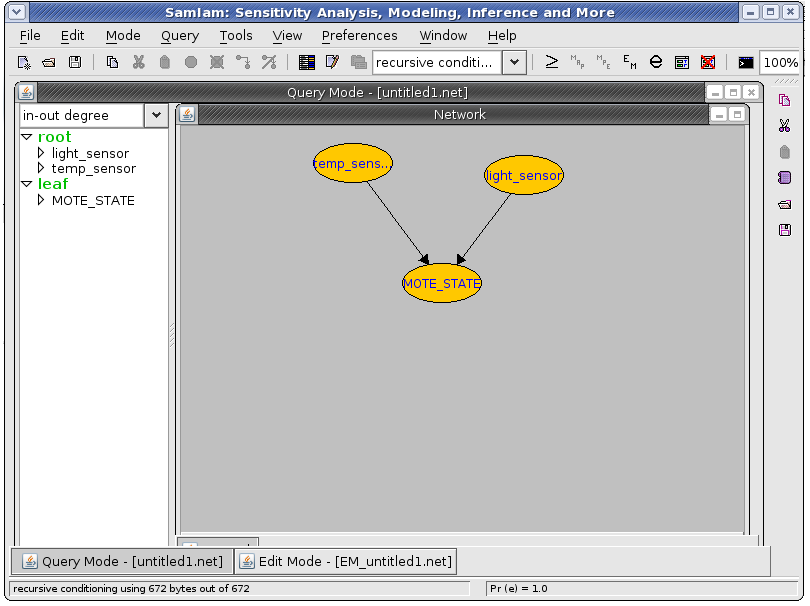
\includegraphics[scale=0.3]	{img/BayesianNetwork.png}
\caption{Bayesian network with independent sensor readings} 
\label{Fig1:BayesianNet}
\end{figure} 


\subsubsection{Bayesian Learning Packages} \label{subsubsec:SamIAm}

A Bayesian learning package allows for the automated estimation of Bayesian
network parameters based on a set of training data.

The Bayesian learning package used during the course of this work is called
SamIam (Sensitivity analysis, modeling, Inference, and more)
\cite{Samiam:2004}.SamIam is a Java-based tool developed at the University of
California at Los Angeles (UCLA) that enables modeling and reasoning with Bayesian
networks.

SamIam uses an expectation-maximization (EM) algorithm
\cite{EMAlgoDempster:1977} to find the Maximum
Likelihood (ML) estimates of the parameters of the Bayesian network.

\subsubsection{Evaluation of Bayesian Inference}

The Bayesian inference approach to Wireless Sensor Network (WSN) data aggregation has
the following advantages over the rule-based approach:

\begin{compactitem}
  \item It is a learning-based approach.
  \item Bayesian inference can
  process previously unspecified combinations of evidence to arrive at a
  hypothesis, thereby making it more flexible than the rule-based approach which
  fails upon encountering input combinations not defined in the rules.
  \item The Bayesian network can potentially be stored on memory far more
  compactly than a large set of rules can.
\end{compactitem} 

Therefore, the Bayesian inference approach was chosen for use.

\subsection{Proof of Concept}\label{subsec:ProofOfConcept}

The implementation of a data aggregation mechanism for sensor data
collected from animals was infeasible because: 
\begin{compactitem}
\item It was beyond the scope of
the lab project.
\item Training data to construct a Bayesian network to model
rat behaviour was unavailable. 
\end{compactitem}

Therefore, a demonstrator called MoteState that read
sensor data
from two sensors and used Bayesian inference to determine the state of the
sensor node was designed. This demonstrator is described in greater detail in
Section \ref{subsec:MoteState}.

The rest of this paper is organised as follows. Section 2 describes the hardware
platform, TinyOS, and the details of the demonstrator application implemented.
Section 3 describes the problems faced. Section 4 describes future work.

\section{Implementation} 

This section starts with a description of the hardware platform used, and is
followed by a description of TinyOS 2.x and the rationale behind using it over
TinyOS 1.x. The last part of this section describes the architecture of, and
steps involved in, developing the demonstrator application.
 
\subsection{Hardware Platform used\\}

 \begin{figure}[h]
\centering
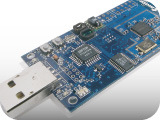
\includegraphics	{img/products-tmotesky-big.jpg}
\caption{The Tmote Sky} 
\label{Fig2:TmoteSky}
\end{figure} 


The hardware platform used for developing MoteState was the Tmote Sky
\cite{TmoteskyDataSheet:2007} (see Figure \ref{Fig2:TmoteSky}). The Tmote Sky
is a wireless sensor node that uses the 16-bit Texas Instruments (TI) MSP430
microcontroller running at 8 MHz, and has 10 kB of RAM, 48 kB of flash, and 128
bytes of information storage. It uses the Chipcon CC2420 802.15.4 compliant
Radio Frequency (RF) transceiver that operates in 2.4 GHz Industrial, Scientific, Medical (ISM) band and allows for a data rate of 250 kbps, and additionally supports TinyOS out of the
box. A Universal Asynchronous Receiver/Transmitter (UART) supports communication between the sensor node and a PC/PDA-based base-station.

\subsection{TinyOS and TinyOS 2.x}

TinyOS \cite{TinyOSManual:2006} is an event-based operating system which is designed for use on sensor nodes. It supports concurrency intensive operations without high hardware requirements. The programming language used to program sensor nodes running TinyOS is Network embedded systems C (NesC), and is an extension of the C programming language. 

TinyOS provides a simulation environment, TinyOS SIMulator (TOSSIM), that provides support for ``offline simulations'' by allowing the running of virtual sensor nodes (``motes'') on a PC. Additionally, applications written for the TinyOS platform are highly portable, as several types of sensor nodes, such as the MICA2 \cite{Mica2DataSheet:2007}, the Tmote Sky \cite{TmoteskyDataSheet:2007}, and the DSYS25z \cite{DSYS25zFlynn:2005} support TinyOS out of the box.

TinyOS 2.0 \cite{TinyOSManual:2006,TinyOS:2006} is a complete redesign and reimplementation of
TinyOS. This was done in order to deal with previously unforeseen
limitations of TinyOS 1.x. Working around these limitations results in tightly
coupled components, hard to find interactions, and a steep learning curve. 

TinyOS 2.0 is not backwards-compatible; i.e., code written for TinyOS 1.x will
not compile on TinyOS 2.0 (though porting code is simple). It has (supposedly) a
less steep learning curve, and performs hardware abstraction using a 3-level
hierarchy. It uses a different boot sequence to TinyOS 1.x, as the boot sequence
only initialises components, and signals the Boot.booted event. The application
component handles the event and starts the appropriate services. It also
supports virtualisation using generic/``instantiable'' components.

\subsection{MoteState} \label{subsec:MoteState}

The MoteState demonstrator was implemented to demonstrate the
applicability of Bayesian learning in WSNs, as described in Section \ref{subsec:ProofOfConcept}.
The application used two
sensors on the Tmote Sky \cite{TmoteskyDataSheet:2007} mote that measure 
temperature and
ambient light. The mote is, at all times, in one of the following five states:

\begin{compactitem}
  \item Inside fridge, with door closed.
  \item Inside fridge, with door open.
  \item In a not-so-well-lit room.
  \item In a well-lit room (or outside in the sun).
  \item In a completely dark room.
\end{compactitem}

Initially, it was planned to have a state to indicate that the mote was in the
freezer. However, it was found that keeping motes inside the freezer resulted in
temperatures falling to levels close to their operating limits. This induced
erratic behaviour, as a result of which the state was eliminated.

The rest of this section describes the steps involved in developing the
MoteState application.

% \begin{figure}[h]
%\centering
%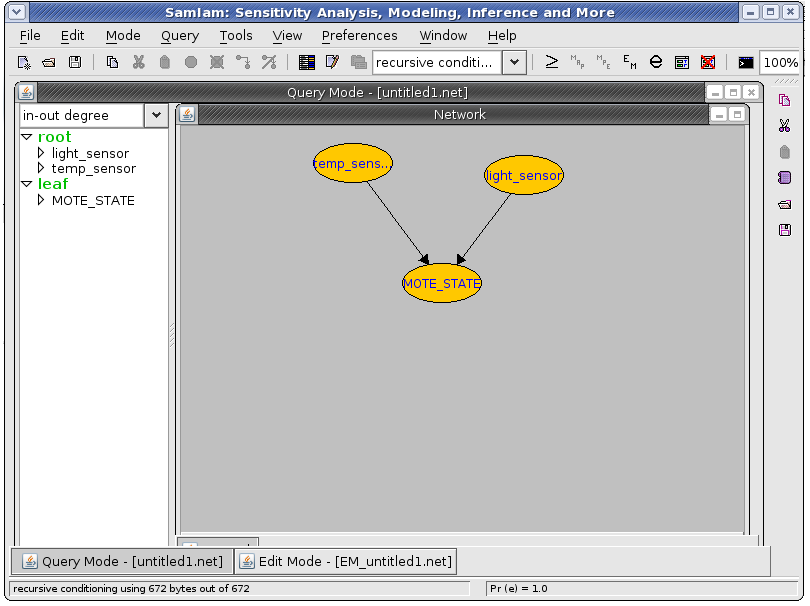
\includegraphics[scale=0.25]{img/BayesianNetwork.png}
%\caption{Bayesian Network constructed} 
%\label{Fig3:BayesianNet}
%\end{figure} 

\subsubsection{Bayesian Network Construction}
\begin{figure}[t]
\centering
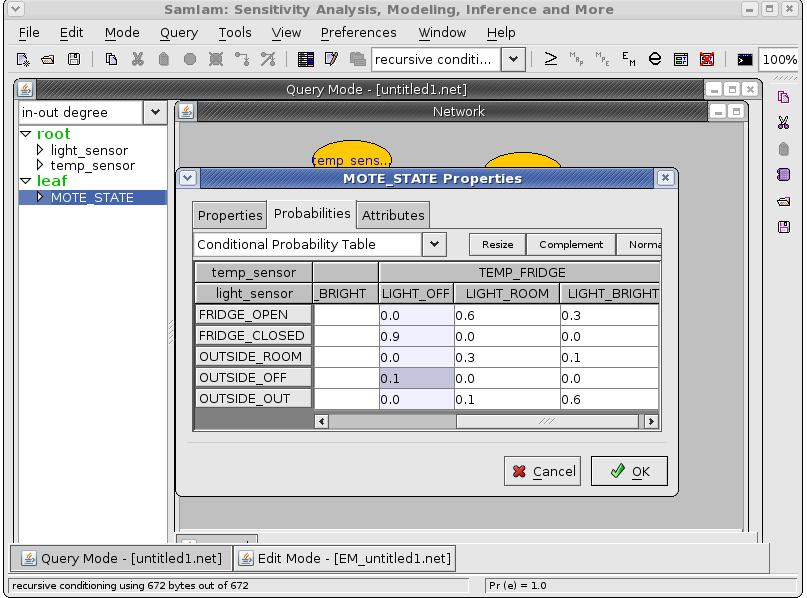
\includegraphics[scale=0.25]{img/SamIAmCondProb.png}
\caption{Conditional Probability Table} 
\label{Fig3:BayesianCondProb}
\end{figure} 
  \begin{figure}[t]
\centering
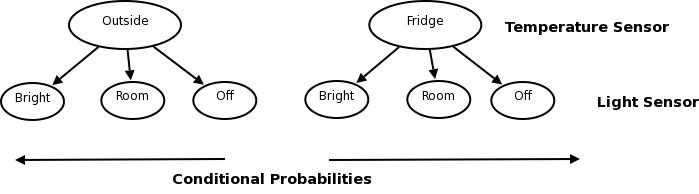
\includegraphics[scale=0.25]{img/SamIamGraph.png}
\caption{Graph structure of conditional probability matrix} 
\label{Fig4:SamIamGraph}
\end{figure}  
A set of training data were created in order to construct a Bayesian network.
The training data is of the form \emph{Temp-sensor, Light-sensor, SNS},
where \emph{Temp-sensor} and \emph{Light-sensor} are states obtained by
clustering sensor readings as described
in Section \ref{subsubsec:Clustering} and Section \ref{subsubsec:MsgTypes}. Appendix \ref{sec:appendixA} contains an example of a training data file.

The training data file was used to construct a Bayesian network using SamIam
\cite{Samiam:2004}  (see Section \ref{subsubsec:SamIAm}). The EM algorithm
\cite{EMAlgoDempster:1977} was used to learn conditional probabilities using the
training data. The Bayesian network constructed is shown in Figure \ref{Fig1:BayesianNet}, and the
conditional probability model obtained upon using the training data  in Figure
\ref{Fig3:BayesianCondProb}.
 
 The conditional probability matrix is a graph, the structure of which is as
 shown in Figure \ref{Fig4:SamIamGraph}.
 



\subsubsection{Message Types} \label{subsubsec:MsgTypes}

The MoteState application uses the following message types:


\subsubsection*{Event Messages}

Event messages are used to transfer event information from the sensor node to the PC base-station. A sensor node transmits an Event message whenever there is a change in the SNS. The Event message is transmitted directly to the PC base-station if the node is directly connected to it (the sink). If not, the Event message is transmitted over a radio link to the sensor node connected to the PC base-station.

An Event message packet (see Figure \ref{Fig7:EventMsgStruct} contains 24 bytes of payload information, including an 8-byte source address, an 8-byte SNS field, and the probability associated with the SNS. The size of the latter two fields can be expanded to include multiple events in a single Event message packet.

  \begin{figure}[h]
\centering
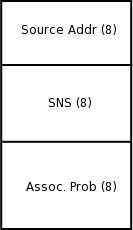
\includegraphics[scale=0.5]{img/EventMsgStruct.png}
\caption{Structure of Event message} 
\label{Fig7:EventMsgStruct}
\end{figure}  

\subsubsection*{Conditional Probability Messages}

Conditional Probability messages are sent from the PC base-station to sensor nodes in the network in order to load a conditional probability model on the sensor node. When a node receives a Conditional Probability message, it broadcasts it to every other node within its radio range.

The structure of the Conditional Probability message may be represented as shown in Figure \ref{Fig8:CondProbMsgStruct}. It contains an 8-byte source address, and a conditional probability matrix, which is a two-dimensional array of size 240 bytes (see Section \ref{subsubsec:CPMRep}).

\begin{figure}[h]
\centering
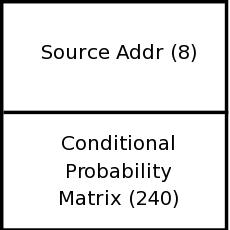
\includegraphics[scale=0.3]{img/CondProbMsgStruct.png}
\caption{Structure of Conditional Probability message} 
\label{Fig8:CondProbMsgStruct}
\end{figure}  

\subsubsection{Clustering} \label{subsubsec:clustering}

Sensor readings are clustered into discrete states as described in
Section \ref{subsubsec:Clustering}. The following thresholds are defined: (1)
\emph{Temp-fridge-threshold}, (2) \emph{Light-off-threshold}, and (3)
\emph{Light-bright-threshold}. This results in two temperature sensor states
(\emph{Temp-fridge} and \emph{Temp-outside}), and three light sensor states
(\emph{Light-bright}, \emph{Light-room}, and \emph{Light-off}).

The light sensor determines a change in state immediately. However, the temperature sensor on the Tmote Sky \cite{TmoteskyDataSheet:2007} takes longer to reflect changes in the ambient temperature. Therefore, the decision on the threshold had to be taken on the basis of an acceptable settling time. Figure \ref{Fig12:TempVsTime} shows the rate of change of the temperature with time. The blue part of the graph shows the node when in a room, the green part shows the time in which the node was placed inside a refrigerator, and the red part shows the time the node was taken out of the refrigerator, and placed in the room again.

\begin{figure}[h]
\centering
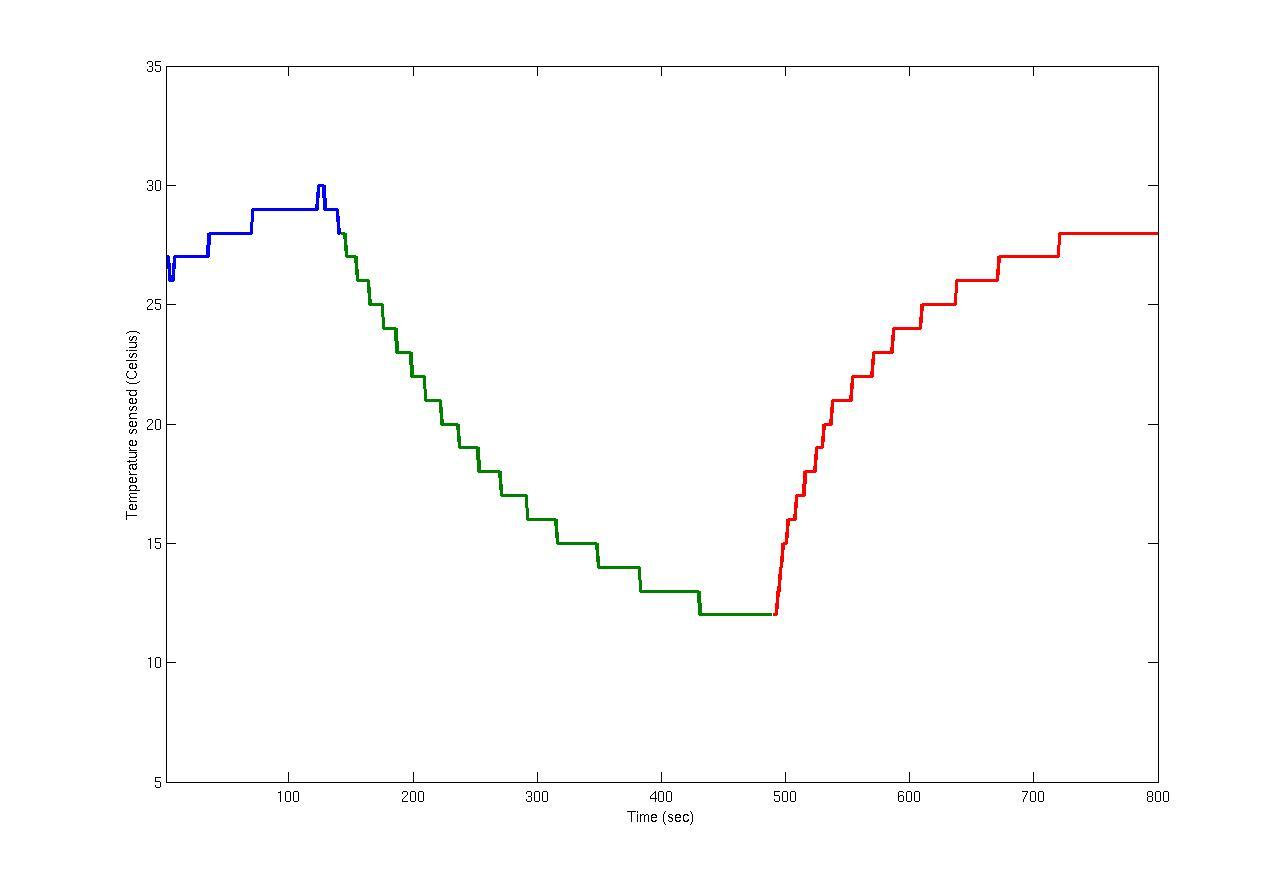
\includegraphics[scale=0.2]{img/tempVsTime.jpg}
\caption{Rate of change of temperature with time} 
\label{Fig12:TempVsTime}
\end{figure}  


It was found that the temperature sensor took almost 10 minutes after the node was placed inside the refrigerator to settle at a temperature. It took a little longer than 8 minutes for the temperature to settle again, upon the node being replaced in the room. Therefore, it was necessary to determine values for the $Temp-fridge$ and $Temp-outside$ thresholds which were higher than the settling temperature. The threshold decided upon was 22$^\circ$C, upon which the time taken for a change in the sensor's state, $St$, upon moving the sensor node in to and out of the refrigerator, fell to around 2 minutes.

\subsubsection{Conditional Probability Matrix Representation} \label{subsubsec:CPMRep}

\begin{figure}[t]
\centering
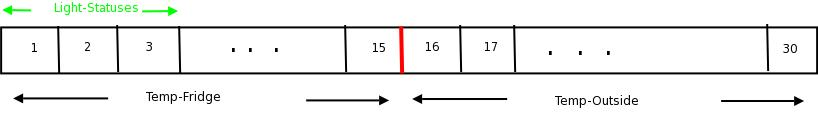
\includegraphics[scale=0.2]{img/CondProbMatrixStruct.png}
\caption{In-code representation of Conditional Probability Matrix} 
\label{Fig9:CondProbMatrixStruct}
\end{figure} 

The conditional probability matrix shown in Figure \ref{Fig3:BayesianCondProb}
is represented in code as a two-dimensional array\footnote{The array was split into two for simplicity of implementation}. The dimensions of the matrix are given by:

\begin{equation}
n_{rows} = n_{ts} \times n_{ls} \\
n_{cols} = n_{sns}
\end{equation}
\noindent
where:
$n_{rows}$ is the number of rows of the conditional probability matrix,\\
\noindent
$n_{cols}$ is the number of columns,\\
\noindent
$n_{ts}$ is the the number of temperature states,\\
\noindent
$n_{ls}$ is the number of light states,and\\
\noindent
$n_{sns}$ is the number of SNSes.

As described in the previous sections, there are two temperature sensor states,
three light sensor states, and five SNSes. As a result, the size of the
conditional probability matrix is $6 \times 5 = 30$ entries. Though probability
values are floating point numbers between 0 and 1, the conditional
probabilities were represented as 7-bit unsigned integers, resulting in a 
conditional probability matrix of size $210$ bits. This was because: (1) 
floating-point variables occupy more memory, and (2) the MSP430 processor on 
the Tmote Sky has no Floating Point Unit (FPU).

The sensor nodes are hard-coded with a conditional probability model, thereby 
allowing it to operate upon start-up without the intervention of the PC 
base-station. However, as described in Section \ref{subsubsec:MsgTypes}, sensor 
nodes can be loaded with an alternate conditional probability model by having 
the PC base-station send a Conditional Probability message to the sink.

Figure \ref{Fig9:CondProbMatrixStruct} shows how the conditional probability 
matrix is stored in memory. As mentioned in the footnote, the array is split in 
two. The first array, to the left of the red line in the figure, shows the 
probability of different SNSes given the temperature sensor is in the first 
state (temp-fridge), The second array, shows the probability of different SNSes 
given the temperature sensor is in the second state.

\subsubsection{Memory Complexity of the Conditional Probability Matrix} \label{subsubsec:CPMMemComplexity}

The memory complexity of the conditional probability matrix can be calculated as follows:\\

\noindent Let $n_{sensor}$ be the number of sensors.\\ \\
\noindent Let $n_{state}$ be the number of states that readings from each 
sensor can be discretised into (assuming each sensor is discretised to the same 
number of states).\\ \\
\noindent Let $n_{sns}$ be the number of states that the sensor node can 
take.\\ \\
\noindent Then, the size of the conditional probability matrix, $size_{cpt}$, 
is equal to:

\begin{equation}
size_{cpt} = n_{state}^{n_{sensor}} \times n_{sns}
\end{equation}

\noindent \\ If $n_{state}$ and $n_{sns}$ are fixed, and $n_{sensor}$ is varied, 
$size_{cpt}$ grows geometrically.\\ \\
\noindent
If $n_{state} = n_{sensor} = size_{cpt} = 4$, 
and 7 bits are required for each element of the matrix, $size_{cpt} = 4^4 
\times 4 * 7 = 7168$ bits = $896$ bytes.

The size of the conditional probability matrix varies logarithmically with the number of sensors as can be seen in Figure . However, if the resolution of the system were to be increased by increasing the number of SNSes, the rise in the size of the matrix is linear (see Figure ).

\begin{figure}[h]
\centering
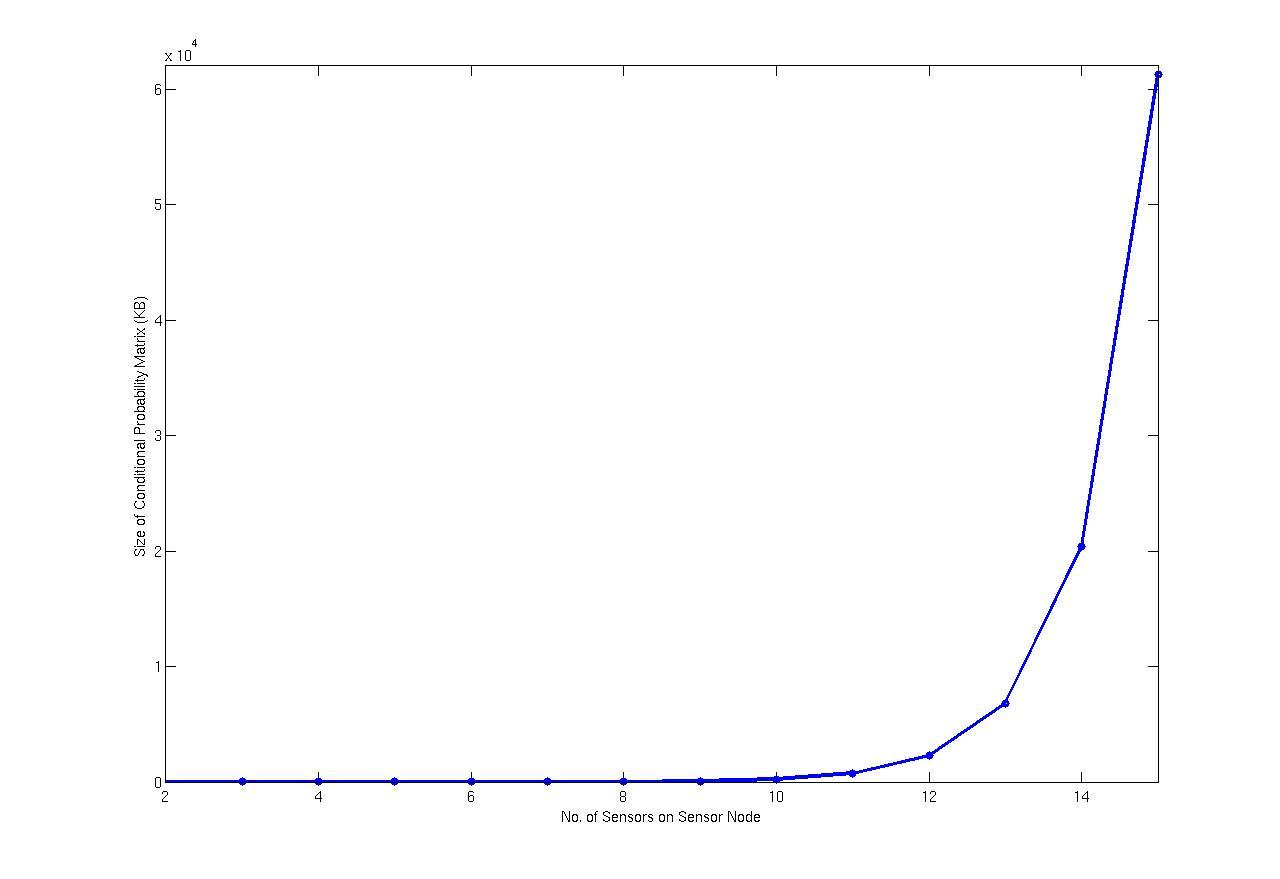
\includegraphics[scale=0.2]{img/SensorVsSize.jpg}
\caption{Conditional probability matrix size vs Number of sensors} 
\label{Fig11:SensorsvsSize}
\end{figure} 
\begin{figure}[h]
\centering
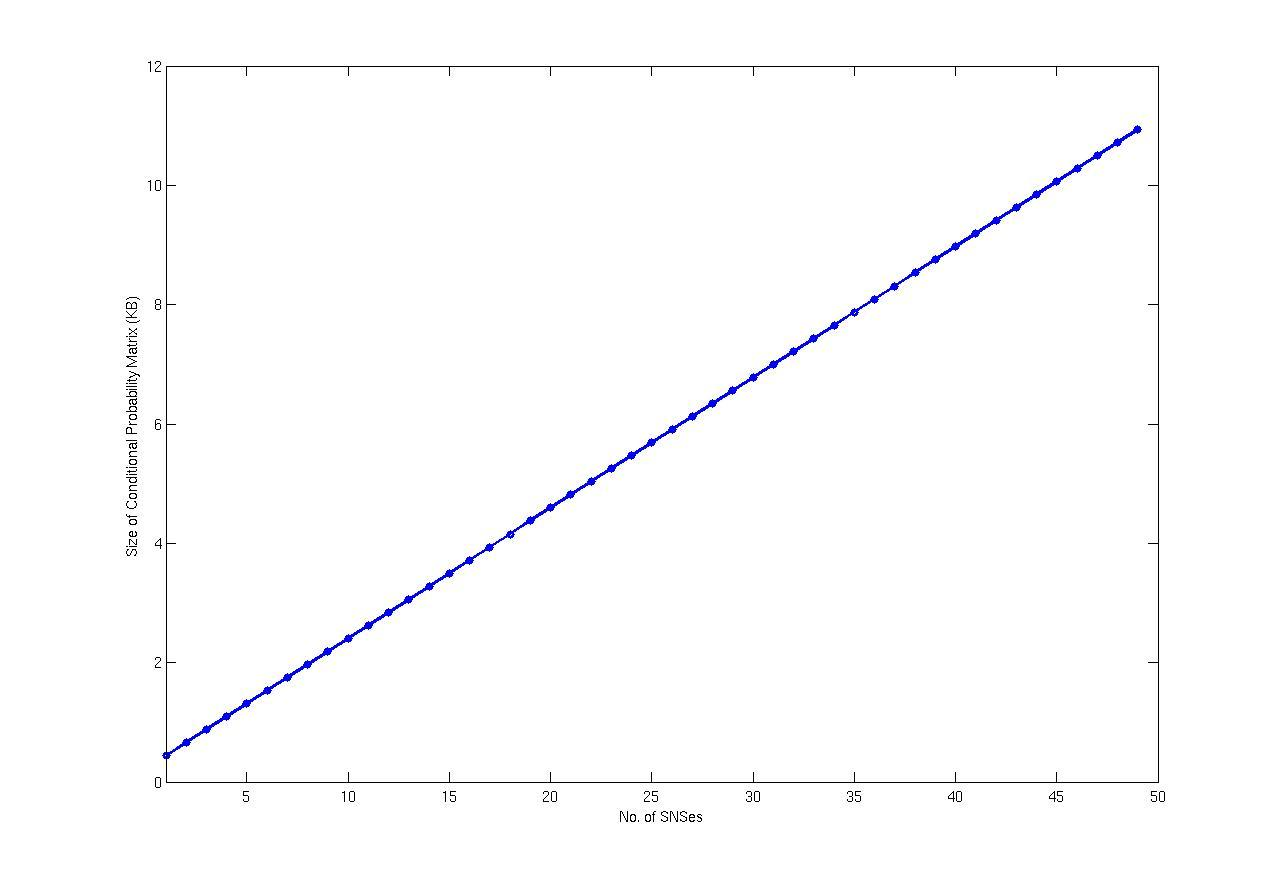
\includegraphics[scale=0.2]{img/SNSVsSize.jpg}
\caption{Conditional probability matrix size vs Number of SNSes} 
\label{Fig10:SNSvsSize}
\end{figure} 


The current structure of the matrix is, therefore, clearly, not scalable. Section \ref{sec:FutureWork} discusses mechanisms to reduce the size of the matrix.


\subsubsection{The MoteState Graphical User Interface}

The MoteState Graphical User Interface (GUI) is Java-based. It provides a graphical
display of the
state of any sensor node in the network (see Figure \ref{Fig5:MoteGUI1}, as well as console-based debug information. It can also be used to send a conditional probability model to the sensor nodes in the network, as shown in Figure \ref{Fig6:MoteGUI2}.

The GUI, written using the JFC Swing API, consists of three tabs. The first tab displays the state of the sensor node currently selected. The drop down box allows for the selection of another sensor node. The GUI currently supports display of state information on only two sensor nodes (see Section \ref{sec:FutureWork} for more information on potential improvements to the GUI). The second tab allows the selection of a file containing a conditional probability matrix. Once a valid conditional probability model has been loaded into the GUI from a file, the user can send the model to the sink as a Conditional Probability message through the UART (see Section \ref{subsubsec:MsgTypes}). The third tab, labelled `Log' allows the user to view information sent from the sink to the PC base-station on the console, and is thus a useful debugging tool.

  \begin{figure}[h]
\centering
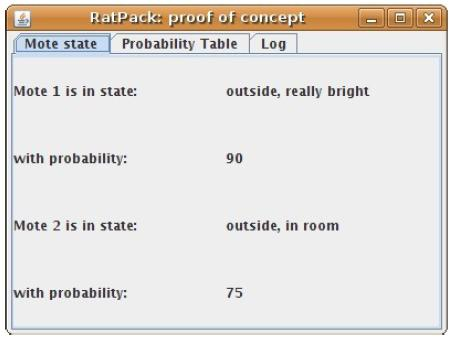
\includegraphics[scale=0.5]{img/MoteGUI1.png}
\caption{Mote state information on MoteState GUI} 
\label{Fig5:MoteGUI1}
\end{figure}  

  \begin{figure}[h]
\centering
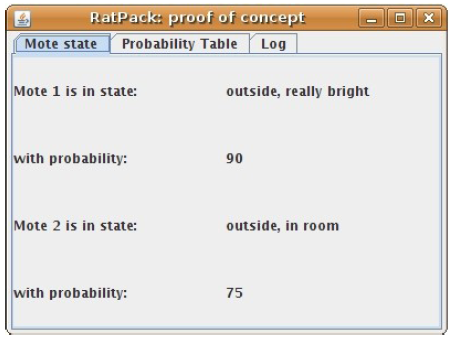
\includegraphics[scale=0.5]{img/MoteGUI2.png}
\caption{Loading Conditional Probability models using the MoteState GUI} 
\label{Fig6:MoteGUI2}
\end{figure}  

\subsection{Implementation Challenges}

Some of the issues faced arose due to the unfamiliarity of the authors with 
Bayesian learning approaches and TinyOS 2.x.

Additionally, determining the structure to be used in order to store the 
conditional probability matrix on the sensor nodes required considerable 
thought. The solution presented is suitable for the number of sensors used for 
the demonstrator. However, the memory requirements for storage of the 
conditional probability model could be much larger if the number of sensors and 
states was increased. Potential solutions to this problem are discussed in 
Section \ref{sec:FutureWork}.

\section{Future Work} \label{sec:FutureWork}

There are several avenues open for future work, some of which are presented 
below:

\subsection{Handling Multiple Sensor Nodes}

The GUI currently supports the display of state information for two sensor 
nodes. Therefore, future work could involve the modification of the GUI to 
support the display of state information from multiple sensor nodes, a trivial 
task.

Additionally, state information is currently transmitted to the sink using a 
simple broadcast mechanism without forwarding. This requires every sensor node 
to be within transmission range of the sink. Therefore, a forwarding mechanism 
may be added to the sensor node implementation.

However, this does not solve the problem of sparse connectivity in a network of 
mobile nodes, where a path may not always exist between a node and the sink. 
Therefore, a line of future work would be 
to investigate routing in networks with intermittent connectivity, thereby 
creating a Disruption-Tolerant Network (DTN) \cite{dtnResourceAllocation:2007}.

Routing protocols for DTNs may be either \emph{epidemic} or \emph{forwarding}. 
In the former, the packet to be forwarded is replicated, whereas in the latter 
only a single copy of the packet is forwarded. However, 
\cite{dtnResourceAllocation:2007} states that most such DTN routing protocols 
cause only incidental improvements in routing metrics such as delivery latency, 
average throughput, and packet delivery ratio. Therefore, the Resource 
Allocation Protocol for Intentional DTN routing (RAPID), an epidemic routing 
protocol that produces intentional improvements in routing metrics, would be a 
protocol worth investigating further.

\subsection{In-mote collection of multiple SNS changes}

The MoteState demonstrator transmits Event messages every time there is a change in the SNS. This can be improved upon by performing one of the following: 
\begin{compactitem}
\item A polling-based system where the sink queries the sensor node, upon which the queried node transmits all the SNS changes since the last poll was performed.
\item The sensor node stores state changes, and transmits it when it is aware of a path to the sink and the time since the last transmission/number of SNS changes exceeds a particular threshold.
\end{compactitem}
\subsection{Reduction of Conditional Probability Matrix size}

As shown in Section \ref{subsubsec:CPMMemComplexity}, the size of the conditional probability matrix grows geometrically with the number of sensors from which readings are collected. In order to reduce the memory requirements, two approaches, which are outlined below, may be taken.

\subsubsection{Precision Reduction}

The precision to which the probabilities are represented in the conditional probability matrix can be reduced in order to reduce memory requirements. Currently, 7-bit unsigned integers are used to represent conditional probabilities (see Section \ref{subsubsec:CPMRep}) as values between 0 and 100. If the precision was reduced by one degree - resulting in a reduction in the range of possible probability values to 10 ($1 \ldots 10$), the number of bits required to represent a probability drops to 4 bits, resulting in a 42\% reduction in the size of the matrix. However, this method results in a loss of precision, and may complicate marginal decisions on SNS.

\subsubsection{Using Coding Techniques}

A coding technique may be used to reduce the size of the conditional probability matrix. Both lossless and lossy coding techniques can be taken into consideration. During the course of this work, two different coding techniques were considered for use in the reduction of the size of the conditional probability matrix; namely, run-length encoding, a lossless scheme, and lossless compression techniques using 2-dimensional Haar wavelets \cite{WaveletsSpaniol:2007}.

The use of a run-length encoding scheme (and thus, by extension, entropy encoding schemes) results in a change in the size of the coded matrix, depending on the conditional probability model used. This is, however, inapplicable, as NesC does not allow for the use of dynamic allocation.

The second method investigated, encoding using 2-dimensional Haar wavelets, was also found to be inapplicable. This was because the averages and details were of the same order. This is illustrated below using a sample conditional probability model. It must be noted that the approach described below works only for square matrices, thereby requiring $n_{state}^{n_{sensor}}$ to be equal to $n_{sns}$.

Let $\mu$ be a conditional probability model defined as:

\begin{equation*}
\mu = \left( \begin{array}{cccc}
0 & 90 & 0 & 40 \\
80 & 0 & 40 & 0 \\
20 & 0 & 60 & 0 \\
0 & 100 & 0 & 60 \end{array}
 \right)
\end{equation*}

The approach taken to perform a 2-dimensional Haar transform on this matrix involves first performing a 1-dimensional Haar transform on each row in turn, resulting in 2 averages and 2 details being produced, as shown below \footnote{The calculated averages are represented in the matrix in bold face.}:

\begin{equation*}
\mu = \left( \begin{array}{cccc}
\textbf{45} & \textbf{20} & -45 & -20 \\
\textbf{40} & \textbf{20} & +40 & +20 \\
\textbf{10} & \textbf{30} & +10 & +30 \\
\textbf{50} & \textbf{30} & -50 & -30 \end{array}
 \right)
\end{equation*}

The second step involves the application of a 1-dimensional Haar transform along the columns of the conditional probability matrix that contain the averages, which, in this case, are the two left-hand columns. This results in the following matrix:

\begin{equation*}
\mu = \left( \begin{array}{cccc}
\textbf{42} & \textbf{20} & -45 & -20 \\
\textbf{30} & \textbf{30} & +40 & +20 \\
+3 & 0 & +10 & +30 \\
-20 & 0 & -50 & -30 \end{array}
 \right)
\end{equation*}

The two steps above are applied recursively, until one global average is obtained, resulting in the matrix below:


\begin{equation*}
\mu = \left( \begin{array}{cccc}
\textbf{30} & +11 & -45 & -20 \\
+1 & 0 & +40 & +20 \\
+8 & 0 & +10 & +30 \\
-20 & 0 & -50 & -30 \end{array}
 \right) 
\end{equation*}

Three problems with this approach are immediately apparent:
\begin{compactitem}
 \item Haar transforms cause a reduction in memory requirements only if the averages are much smaller than the details. This is clearly not the case here, as the averages and details are values of the same order.

\item Additionally, 2-dimensional Haar transforms are lossy, and results in the loss of data. The matrix, when reconstructed from the 2-dimensional Haar transform is:

\begin{equation*}
\mu ' = \left( \begin{array}{cccc}
0 & 90 & 0 & 40 \\
79 & -1 & 40 & 0 \\
19 & -1 & 59 & -1 \\
-1 & 99 &-1 & 59 \end{array}
 \right)
\end{equation*}

\end{compactitem}

\subsection{Improving Responsiveness}

As discussed in Section \ref{subsubsec:clustering}, the time taken for the temperature sensor to fall below the defined threshold was around 2 minutes when the $temp-outside$ and $temp-fridge$ thresholds were set to 22$^\circ$C. However, this threshold was determined arbitrarily, and may not be as appropriate if the ambient temperature were different. Additionally, for certain applications, the system's current responsiveness may be inadequate. Therefore, an approach would be to replace the rigidly defined thresholds, and use a mechanism to change the sensor state $St$ when \emph{the rate of change} of the sensor value exceeds a particular threshold.

\bibliography{references}
\bibliographystyle{abbrv}

%% ADDED TO INTEGRATE BIBLIOGRAPHY INTO TEX FILE

%% ADDED TO INTEGRATE BIBLIOGRAPHY INTO TEX FILE

%\pagebreak
%\balancecolumns
\appendix

\section{Training Data} \label{sec:appendixA}

The training data used to generate (one of) the conditional probability model(s) used by the MoteState demonstrator are presented below.
\begin{center}
\begin{mylisting}
\begin{verbatim}
light_sensor,temp_sensor,MOTE_STATE
LIGHT_ROOM,TEMP_FRIDGE,FRIDGE_OPEN
LIGHT_OFF,TEMP_FRIDGE,FRIDGE_CLOSED
LIGHT_OFF,TEMP_OUTSIDE,OUTSIDE_OUT
LIGHT_ROOM,TEMP_FRIDGE,FRIDGE_OPEN
LIGHT_OFF,TEMP_FRIDGE,FRIDGE_CLOSED
LIGHT_ROOM,TEMP_OUTSIDE,OUTSIDE_OUT
LIGHT_OFF,TEMP_OUTSIDE,OUTSIDE_OFF
LIGHT_ROOM,TEMP_OUTSIDE,FRIDGE_OPEN
LIGHT_BRIGHT,TEMP_OUTSIDE,FRIDGE_OPEN
LIGHT_OFF,TEMP_FRIDGE,FRIDGE_CLOSED
LIGHT_ROOM,TEMP_FRIDGE,FRIDGE_OPEN
LIGHT_OFF,TEMP_OUTSIDE,FRIDGE_CLOSED
LIGHT_BRIGHT,TEMP_FRIDGE,OUTSIDE_OUT
LIGHT_OFF,TEMP_OUTSIDE,OUTSIDE_OUT
LIGHT_OFF,TEMP_OUTSIDE,OUTSIDE_OFF
LIGHT_OFF,TEMP_OUTSIDE,OUTSIDE_OFF
LIGHT_BRIGHT,TEMP_FRIDGE,FRIDGE_OPEN
LIGHT_BRIGHT,TEMP_OUTSIDE,OUTSIDE_OUT
LIGHT_BRIGHT,TEMP_OUTSIDE,FRIDGE_OPEN
LIGHT_OFF,TEMP_OUTSIDE,OUTSIDE_OFF
LIGHT_ROOM,TEMP_FRIDGE,FRIDGE_OPEN
LIGHT_ROOM,TEMP_OUTSIDE,OUTSIDE_ROOM
LIGHT_OFF,TEMP_OUTSIDE,FRIDGE_CLOSED
LIGHT_BRIGHT,TEMP_OUTSIDE,FRIDGE_OPEN
LIGHT_ROOM,TEMP_OUTSIDE,OUTSIDE_ROOM
LIGHT_BRIGHT,TEMP_FRIDGE,OUTSIDE_OUT
LIGHT_OFF,TEMP_FRIDGE,OUTSIDE_OFF
LIGHT_ROOM,TEMP_FRIDGE,FRIDGE_OPEN
LIGHT_BRIGHT,TEMP_OUTSIDE,OUTSIDE_ROOM
LIGHT_ROOM,TEMP_OUTSIDE,FRIDGE_OPEN
LIGHT_OFF,TEMP_OUTSIDE,OUTSIDE_OFF
LIGHT_ROOM,TEMP_FRIDGE,OUTSIDE_OUT
LIGHT_OFF,TEMP_FRIDGE,FRIDGE_CLOSED
LIGHT_OFF,TEMP_FRIDGE,FRIDGE_CLOSED
LIGHT_OFF,TEMP_FRIDGE,FRIDGE_CLOSED
LIGHT_OFF,TEMP_FRIDGE,FRIDGE_CLOSED
LIGHT_BRIGHT,TEMP_OUTSIDE,OUTSIDE_OUT
LIGHT_OFF,TEMP_OUTSIDE,OUTSIDE_OUT
LIGHT_BRIGHT,TEMP_FRIDGE,FRIDGE_OPEN
LIGHT_OFF,TEMP_OUTSIDE,FRIDGE_CLOSED
LIGHT_OFF,TEMP_FRIDGE,FRIDGE_CLOSED
LIGHT_ROOM,TEMP_OUTSIDE,OUTSIDE_ROOM
LIGHT_BRIGHT,TEMP_OUTSIDE,FRIDGE_OPEN
LIGHT_OFF,TEMP_OUTSIDE,FRIDGE_CLOSED
LIGHT_OFF,TEMP_OUTSIDE,OUTSIDE_OFF
LIGHT_OFF,TEMP_FRIDGE,FRIDGE_CLOSED
LIGHT_ROOM,TEMP_OUTSIDE,OUTSIDE_ROOM
LIGHT_ROOM,TEMP_OUTSIDE,OUTSIDE_ROOM
LIGHT_ROOM,TEMP_OUTSIDE,FRIDGE_OPEN
LIGHT_ROOM,TEMP_OUTSIDE,FRIDGE_OPEN
LIGHT_OFF,TEMP_OUTSIDE,FRIDGE_CLOSED
LIGHT_ROOM,TEMP_OUTSIDE,FRIDGE_OPEN
LIGHT_OFF,TEMP_OUTSIDE,OUTSIDE_OFF
LIGHT_ROOM,TEMP_FRIDGE,FRIDGE_OPEN
LIGHT_OFF,TEMP_OUTSIDE,FRIDGE_CLOSED
LIGHT_OFF,TEMP_OUTSIDE,FRIDGE_CLOSED
LIGHT_OFF,TEMP_OUTSIDE,OUTSIDE_OFF
LIGHT_OFF,TEMP_OUTSIDE,FRIDGE_CLOSED
LIGHT_OFF,TEMP_OUTSIDE,FRIDGE_CLOSED
LIGHT_BRIGHT,TEMP_FRIDGE,OUTSIDE_OUT
\end{verbatim}
\end{mylisting}
\end{center}
   

\section{Acknowledgements}

The authors would like to thank Dipl. Inf. Jo Agila Bitsch Link, Research 
Assistant, Lehrstuhl f\"ur Informatik, RWTH Aachen, for his constant guidance 
and support throughout the development of this work and the writing of this 
report. The authors would also like to thank M. Comp.Sc. Olaf Landsiedel, 
Research Assistant, Lehrstuhl f\"ur Informatik and Prof. Dr-Ing. Klaus Wehrle, Head, 
Distributed Systems Group, Lehrstuhl f\"ur Informatik, RWTH Aachen, for their 
advice and guidance throughout the period this course was offered. This section 
would be incomplete without a word of thanks to Vaishak Belle, Lehrstuhl f\"ur 
Informatik, RWTH Aachen, who helped immeasurably with references for, and 
explanatory notes on Bayesian and Rule-based inference, and aided in the search 
for a Bayesian learning package. Anand Kulkarni, Graduate Student, University of
California at Berkeley is also owed the authors' gratitude for his invaluable 
suggestions on improving the paper.
 
\section{List of Abbreviations}

\begin{quote}
\begin{tabular}{|c|c|}
\hline
WSN & Wireless Sensor Network \\
\hline 
SNS & Sensor Node State\\ 
\hline
SamIam & Sensitivity analysis, modeling,\\
  & Inference, and more \\
  \hline
RF & Radio Frequency\\
\hline
ISM & Industrial, Scientific, Medical \\
\hline
UART & Universal Asynchronous \\
 & Receiver/Transmitter \\
 \hline
NesC & Network embedded systems C \\
\hline
TOSSIM & TinyOS Simulator \\
\hline
CPM & Conditional Probability Matrix \\
\hline
GUI & Graphical User Interface \\
\hline
\end{tabular}
\end{quote}

\section{List of Symbols}

\begin{quote}
\begin{tabular}{|c|c|}
\hline
$n_{sensor}$ & number of sensors \\
\hline 
$S_i$ & $i^{th}$ sensor on a sensor node \\
\hline 
$St_{lm}$ & Sensor state assigned to \\
 & readings in the interval $[x_l,x_m]$ \\
 \hline 
$H_0$ & Hypothesis \\
\hline 
$P(H_0)$ & Posterior probability $H_0$ \\
\hline 
$e$ & Observed Evidence \\
\hline 
$P(e)$ & Marginal probability of e \\
\hline 
$P(H_0|e)$ & Conditional probability of \\ 
 &  truth of hypothesis \\
\hline
$E$ & Set of independent \\
 & evidences $[e_i|i=1 \ldots N_{ev}]$ \\
 \hline 
$N_{ev}$ & Number of independent evidences \\
\hline 
$\lambda$ & Given set of sensor readings \\
\hline 
$SNS_{\alpha}$ & Given SNS \\
\hline 
$n_{rows}$ & Number of rows in CPM \\
\hline 
$n_{cols}$ & Number of columns in CPM \\
\hline 
$n_{ts}$ & Number of temperature states \\
\hline 
$n_{sns}$ & Number of SNSes \\
\hline  
 \end{tabular}
\end{quote}
\balancecolumns
\begin{quote}
\begin{tabular}{|c|c|} 
 \hline
FPU & Floating Point Unit \\
\hline 
$size_{cpt}$ & Size of Conditional probability\\
\hline 
 & matrix.\\
 \hline 
$n_{state}$ & Number of states a sensor node \\
 & can take.\\
\hline
\end{tabular}
\end{quote}

\section{List of Figures}

\begin{quote}
\begin{tabular}{cc}
Bayesian network with independent  &  \\
sensor readings & 3\\ \\
The Tmote Sky & 4\\ \\
Conditional Probability Table & 5\\ \\
Graph structure of Conditional & \\
 Probability Matrix & 5 \\ \\
Structure of Event message & 5 \\ \\
Structure of Conditional  & \\
Probability message & 5 \\ \\
 \end{tabular}
\end{quote}
\balancecolumns
\begin{quote}
\begin{tabular}{cc} 
Rate of change of & \\
temperature with time & 6 \\ \\
In-code representation of  &  \\ 
 Conditional Probability Matrix & 6 \\ \\
Conditional Probability Matrix size & \\
vs Number of sensors & 7 \\ \\
Conditional Probability Matrix size & \\
vs Number of SNSes & 7 \\ \\
Mote state information on & \\
 MoteState GUI & 7\\ \\
Loading Conditional Probability & \\
 models using the MoteState GUI & 7 \\ \\ 
\end{tabular}
\end{quote}

\end{document}
